\documentclass[11pt]{article}

\usepackage[utf8]{inputenc}
\usepackage[T1]{fontenc}
\usepackage{lmodern}
\usepackage[margin=1in]{geometry}
\usepackage{setspace}
\usepackage{booktabs}
\usepackage{longtable}
\usepackage{array}
\usepackage{enumitem}
\usepackage{hyperref}
\usepackage{xcolor}
\usepackage{graphicx}
\usepackage{float}

\hypersetup{
    colorlinks=true,
    linkcolor=blue,
    urlcolor=blue,
    pdftitle={Week 5 - Representation and Dimensionality Report},
    pdfauthor={MovieLens Discovery Project Team}
}

\setstretch{1.08}
\setlength{\parskip}{0.5em}
\setlength{\parindent}{0pt}

\title{Week 5 - Representation and Dimensionality Report}
\date{April 2026}

\begin{document}

\maketitle

\section{Executive Summary}

This report documents the Week 5 deliverables for representation and dimensionality reduction. The objective is to move from cleaned MovieLens tables to meaningful feature matrices, then validate structure and redundancy through PCA/SVD and supporting visualizations.

\begin{itemize}[leftmargin=1.5em]
    \item \textbf{Project title}: Personalized Movie Discovery and Recommendation Engine (MovieLens 25M)
    \item \textbf{Course}: Semester Project: Domain Discovery, Recommendation, and Graph Intelligence
    \item \textbf{Milestone objective}: Build reproducible feature representations and dimensionality reduction artifacts
    \item \textbf{Report date}: April 2026
    \item \textbf{Status}: Feature matrices, dimensionality reduction, comparison table, and visualizations completed
\end{itemize}

\section{Feature Matrices}

Two feature matrices are built at the movie level.

\subsection{Numeric and Categorical Matrix}

\textbf{Description}

This matrix combines rating aggregates, time-span coverage, and one-hot genres. It captures overall popularity, rating distribution, and catalog category signals in a compact numeric form.

\textbf{Core columns}

\begin{itemize}[leftmargin=1.5em]
    \item Ratings: \texttt{rating\_count}, \texttt{rating\_mean}, \texttt{rating\_std}, \texttt{rating\_min}, \texttt{rating\_max}, \texttt{rating\_median}
    \item Temporal: \texttt{rating\_first\_ts}, \texttt{rating\_last\_ts}, \texttt{rating\_span\_days}
    \item Categorical: one-hot genre columns derived from \texttt{movie\_genres}
    \item Tag activity: \texttt{tag\_count} (count of distinct tags per movie)
\end{itemize}

\textbf{Output}

\begin{itemize}[leftmargin=1.5em]
    \item \texttt{data/processed/week05/movie\_numeric\_features.parquet}
\end{itemize}

\subsection{Text Matrix (TF-IDF)}

\textbf{Description}

This matrix represents the semantic profile of each movie using aggregated tags and titles. We concatenate \texttt{title} and the unique tag list, then apply TF-IDF with English stop-word removal.

\textbf{TF-IDF configuration}

\begin{itemize}[leftmargin=1.5em]
    \item \texttt{max\_features = 5000}
    \item \texttt{min\_df = 2}
    \item \texttt{stop\_words = "english"}
\end{itemize}

\textbf{Outputs}

\begin{itemize}[leftmargin=1.5em]
    \item \texttt{data/processed/week05/movie\_text\_tfidf.npz}
    \item \texttt{data/processed/week05/movie\_text\_tfidf\_vocab.json}
\end{itemize}

\subsection{Data Sources}

\begin{itemize}[leftmargin=1.5em]
    \item \texttt{data/processed/week03\_v1/movies\_catalog.parquet}
    \item \texttt{data/processed/week03\_v1/movie\_genres.parquet}
    \item \texttt{data/processed/week03\_v1/ratings\_clean.parquet}
    \item \texttt{data/processed/week03\_v1/tags\_clean.parquet}
\end{itemize}

\section{Dimensionality Reduction}

\subsection{PCA (Numeric Matrix)}

\begin{itemize}[leftmargin=1.5em]
    \item Input: standardized numeric matrix
    \item Target variance: 90\% cumulative variance
    \item Output: \texttt{data/processed/week05/movie\_pca\_embeddings.parquet}
    \item Artifact: \texttt{artifacts/week05/pca\_variance.csv}
\end{itemize}

\subsection{Truncated SVD (Text TF-IDF)}

\begin{itemize}[leftmargin=1.5em]
    \item Input: sparse TF-IDF matrix
    \item Components: 200
    \item Output: \texttt{data/processed/week05/movie\_svd\_embeddings.parquet}
    \item Artifact: \texttt{artifacts/week05/svd\_variance.csv}
\end{itemize}

\subsection{t-SNE (Visualization)}

\begin{itemize}[leftmargin=1.5em]
    \item Input: PCA embeddings
    \item Output: \texttt{artifacts/week05/pca\_tsne.parquet}
\end{itemize}

\section{Comparison Table}

\begin{table}[h]
\centering
\begin{tabular}{lccc}
\toprule
Method & Components & Cumulative Variance & Reconstruction Error \\
\midrule
PCA & 20 & 0.9012 & 0.0988 \\
TruncatedSVD & 200 & 0.3572 & 0.6373 \\
\bottomrule
\end{tabular}
\caption{Dimensionality reduction comparison summary from \texttt{artifacts/week05/comparison\_table.csv}.}
\end{table}

\section{Visualization Set}

The Plotly figures are exported to HTML and PNG.

\begin{itemize}[leftmargin=1.5em]
    \item \texttt{artifacts/week05/pca\_cumulative\_variance.html}
    \item \texttt{artifacts/week05/svd\_cumulative\_variance.html}
    \item \texttt{artifacts/week05/tsne\_scatter.html}
\end{itemize}

\begin{figure}[H]
\centering
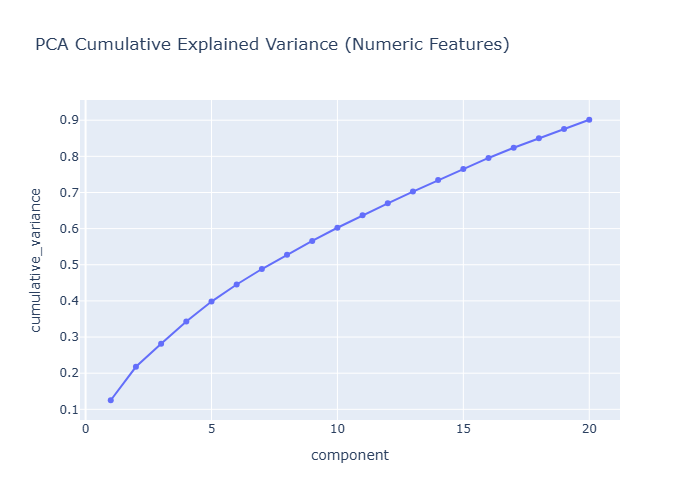
\includegraphics[width=0.8\textwidth]{../../artifacts/week05/pca_cumulative_variance.png}
\caption{PCA cumulative explained variance.}
\end{figure}

\begin{figure}[H]
\centering
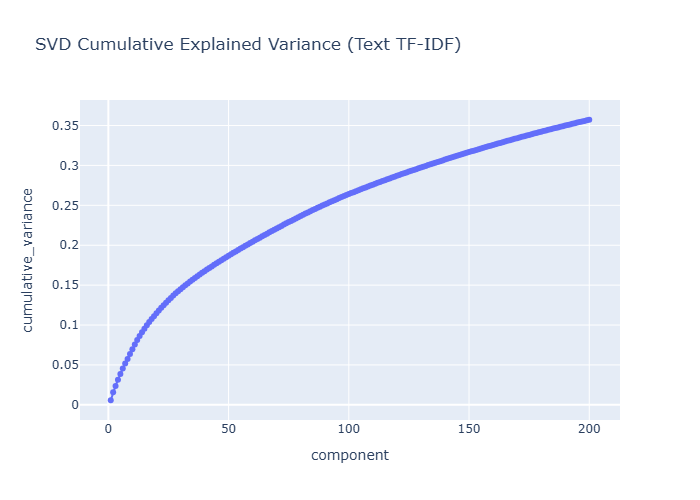
\includegraphics[width=0.8\textwidth]{../../artifacts/week05/svd_cumulative_variance.png}
\caption{SVD cumulative explained variance.}
\end{figure}

\begin{figure}[H]
\centering
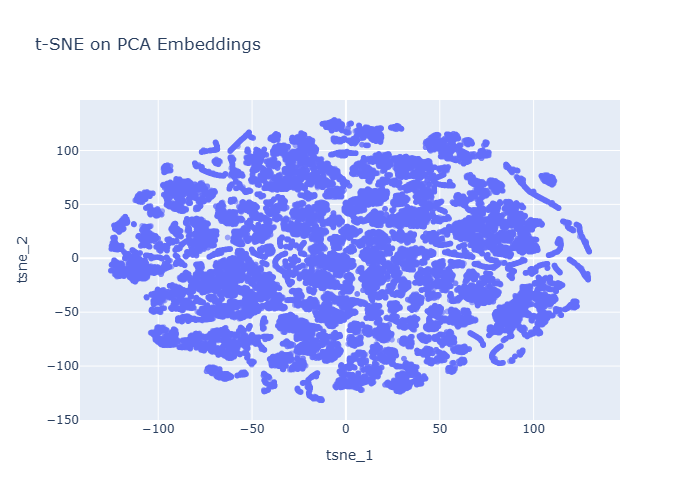
\includegraphics[width=0.8\textwidth]{../../artifacts/week05/tsne_scatter.png}
\caption{t-SNE scatter on PCA embeddings.}
\end{figure}

\section{Technical Interpretation}

\begin{enumerate}[leftmargin=1.5em]
    \item \textbf{Numeric features are compact}: PCA captures 90.12\% of numeric-feature variance with 20 components, indicating strong redundancy among rating statistics and genre indicators.
    \item \textbf{Text features are diffuse}: Truncated SVD reaches 35.72\% cumulative variance at 200 components, reflecting higher semantic diversity across tags and titles.
    \item \textbf{Representation trade-off}: Numeric signals compress well, while text signals preserve more long-tail variation; downstream models should treat these spaces differently.
\end{enumerate}

\section{Reproducibility}

To rebuild all Week 5 outputs:

\begin{verbatim}
python3 scripts/build_week05_pipeline.py
\end{verbatim}

\end{document}
